%----------------------------------------------------------------------------------------
%	PACKAGES AND OTHER DOCUMENT CONFIGURATIONS
%----------------------------------------------------------------------------------------

\documentclass{article}

\usepackage{fancyhdr} % Required for custom headers
\usepackage{lastpage} % Required to determine the last page for the footer
\usepackage{extramarks} % Required for headers and footers
\usepackage{graphicx} % Required to insert images
\usepackage{listings}
\usepackage{color}
\usepackage{xcolor}
\usepackage{caption}
\usepackage{enumitem}
\usepackage{amsmath}
\usepackage{tikz}
\usepackage{parcolumns}
\usetikzlibrary{calc,shapes.multipart,chains,arrows}

\DeclareCaptionFont{white}{\color{white}}
\DeclareCaptionFormat{listing}{%
\parbox{\textwidth}{\colorbox{gray}{\parbox{\textwidth}{#1#2#3}}\vskip-4pt}}
\captionsetup[lstlisting]{format=listing,labelfont=white,textfont=white}

% Margins
\topmargin=-0.45in
\evensidemargin=0in
\oddsidemargin=0in
\textwidth=6.5in
\textheight=9.0in
\headsep=0.25in 

\linespread{1.1} % Line spacing

% Set up the header and footer
\pagestyle{fancy}
%\lhead{\hmwkAuthorName} % Top left header
%\chead{\hmwkClass\ (\hmwkClassInstructor\ \hmwkClassTime): \hmwkTitle} % Top center header
%\rhead{\hmwkDueDate} % Top right header
\lfoot{\lastxmark} % Bottom left footer
\cfoot{} % Bottom center footer
\rfoot{Page\ \thepage\ of\ \pageref{LastPage}} % Bottom right footer
\renewcommand\headrulewidth{0.4pt} % Size of the header rule
\renewcommand\footrulewidth{0.4pt} % Size of the footer rule

\setlength\parindent{0pt} % Removes all indentation from paragraphs

%----------------------------------------------------------------------------------------
%	DOCUMENT STRUCTURE COMMANDS
%	Skip this unless you know what you're doing
%----------------------------------------------------------------------------------------

\setcounter{secnumdepth}{0} % Removes default section numbers
\newcounter{homeworkProblemCounter} % Creates a counter to keep track of the number of problems

\newcommand{\homeworkProblemName}{}
\newenvironment{homeworkProblem}[1][Problem \arabic{homeworkProblemCounter}]{ % Makes a new environment called homeworkProblem which takes 1 argument (custom name) but the default is "Problem #"
\stepcounter{homeworkProblemCounter} % Increase counter for number of problems
\renewcommand{\homeworkProblemName}{#1} % Assign \homeworkProblemName the name of the problem
\section{\homeworkProblemName} % Make a section in the document with the custom problem count
}

%----------------------------------------------------------------------------------------
%   COLORS AND LANGUAGAGE
%----------------------------------------------------------------------------------------

\lstset{
    frame=lrb,xleftmargin=\fboxsep,xrightmargin=-\fboxsep,language=Java,basicstyle=\ttfamily,
    breaklines=true,columns=fullflexible,keepspaces=true,escapeinside={\%*}{*)}
       }

%----------------------------------------------------------------------------------------
%	NAME AND CLASS SECTION
%----------------------------------------------------------------------------------------

%\newcommand{\hmwkTitle}{Homework\ \#1} % Assignment title
%\newcommand{\hmwkDueDate}{Wednesday,\ January\ 28,\ 2015} % Due date
%\newcommand{\hmwkClass}{COP\ 5621} % Course/class
%\newcommand{\hmwkClassTime}{6:25pm} % Class/lecture time
%\newcommand{\hmwkClassInstructor}{Smith} % Teacher/lecturer
%\newcommand{\hmwkAuthorName}{Musa V. Ahmed \& Jose Acosta} % Your name

%----------------------------------------------------------------------------------------

\begin{document}
\belowcaptionskip=-10pt

%----------------------------------------------------------------------------------------
%	PROBLEM 1
%----------------------------------------------------------------------------------------

\section{10s}
    \noindent\begin{minipage}{.45\textwidth}
    \lstinputlisting[basicstyle=\ttfamily\scriptsize,frame=none]{set_a_10s/tc_changes_timestamps_set_a_10s.out}
    \end{minipage}\hfill
    \begin{minipage}{.45\textwidth}
    \lstinputlisting[basicstyle=\ttfamily\scriptsize,frame=none]{set_a_10s/iperf_set_a_10s.out}
    \end{minipage}
    
    \begin{center}
        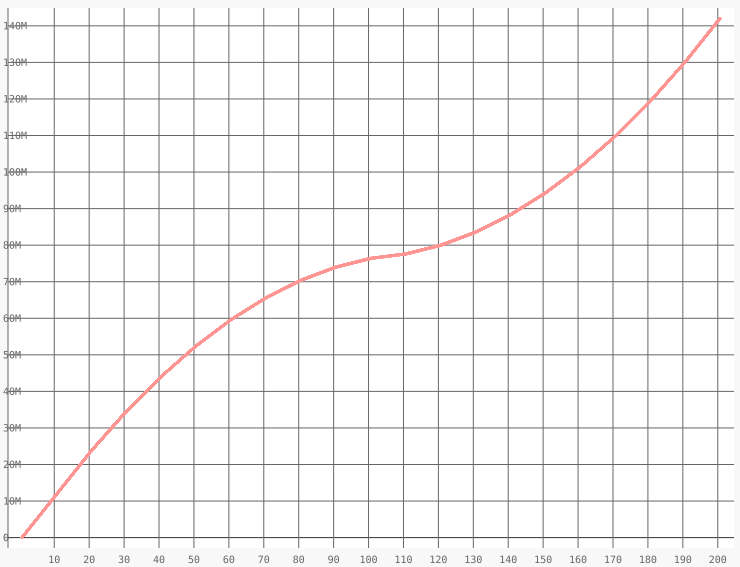
\includegraphics[angle=90]{set_a_10s/set_a_10s.png}
    \end{center}
\clearpage

\section{5s}
    \noindent\begin{minipage}{.45\textwidth}
    \lstinputlisting[basicstyle=\ttfamily\scriptsize,frame=none]{set_a_5s/tc_changes_timestamps_set_a_5s.out}
    \end{minipage}\hfill
    \begin{minipage}{.45\textwidth}
    \lstinputlisting[basicstyle=\ttfamily\scriptsize,frame=none]{set_a_5s/iperf_set_a_5s.out}
    \end{minipage}
    
    \begin{center}
    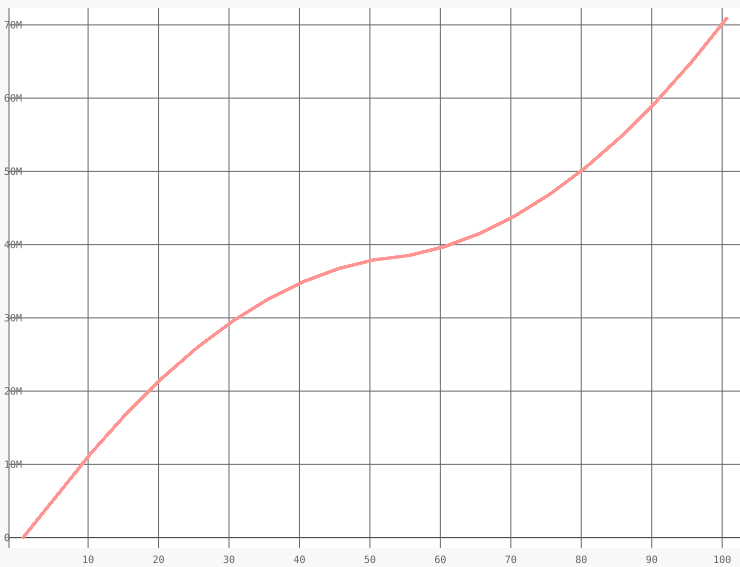
\includegraphics[angle=90]{set_a_5s/set_a_5s.png}
    \end{center}
\clearpage

\section{2.5s}
    \noindent\begin{minipage}{.45\textwidth}
    \lstinputlisting[basicstyle=\ttfamily\scriptsize,frame=none]{set_a_2.5s/tc_changes_timestamps_set_a_2.5s.out}
    \end{minipage}\hfill
    \begin{minipage}{.45\textwidth}
    \lstinputlisting[basicstyle=\ttfamily\scriptsize,frame=none]{set_a_2.5s/iperf_set_a_2.5s.out}
    \end{minipage}
    
    \begin{center}
    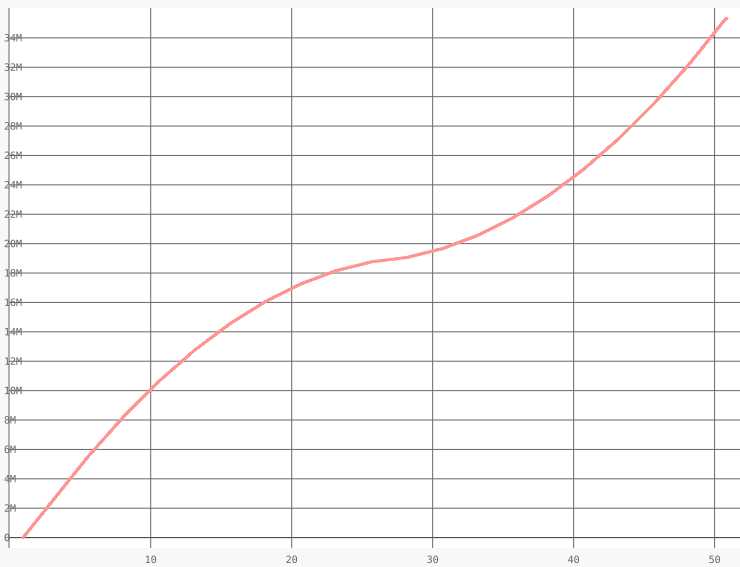
\includegraphics[angle=90]{set_a_2.5s/set_a_2_5s.png}
    \end{center}
\clearpage

\section{1s}
    \noindent\begin{minipage}{.45\textwidth}
    \lstinputlisting[basicstyle=\ttfamily\scriptsize,frame=none]{set_a_1s/tc_changes_timestamps_set_a_1s.out}
    \end{minipage}\hfill
    \begin{minipage}{.45\textwidth}
    \lstinputlisting[basicstyle=\ttfamily\scriptsize,frame=none]{set_a_1s/iperf_set_a_1s.out}
    \end{minipage}
    
    \begin{center}
    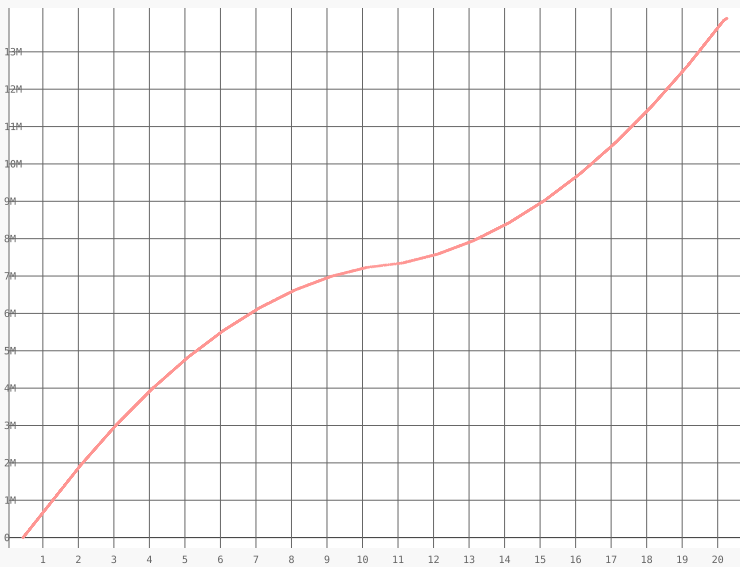
\includegraphics[angle=90]{set_a_1s/set_a_1s.png}
    \end{center}
\clearpage

\section{0.75s}
    \noindent\begin{minipage}{.45\textwidth}
    \lstinputlisting[basicstyle=\ttfamily\scriptsize,frame=none]{set_a_0.75s/tc_changes_timestamps_set_a_0.75s.out}
    \end{minipage}\hfill
    \begin{minipage}{.45\textwidth}
    \lstinputlisting[basicstyle=\ttfamily\scriptsize,frame=none]{set_a_0.75s/iperf_set_a_0.75s.out}
    \end{minipage}
    
    \begin{center}
    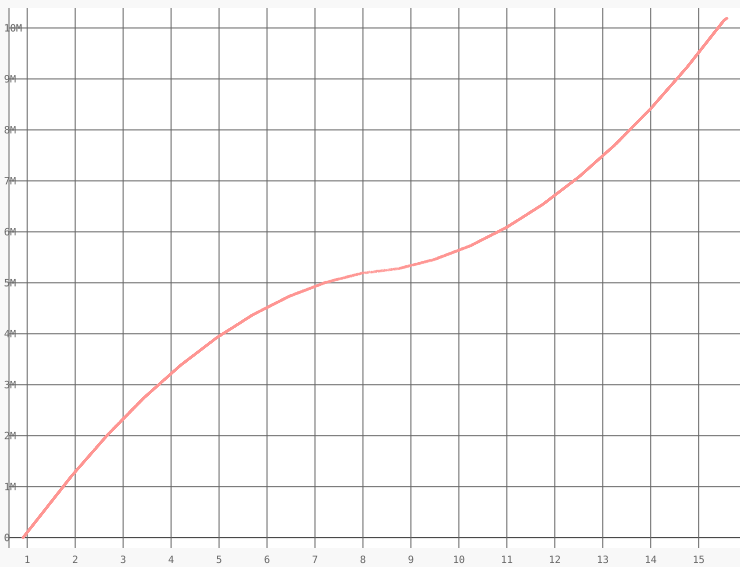
\includegraphics[angle=90]{set_a_0.75s/set_a_0_75s.png}
    \end{center}
\clearpage

\section{0.5s}
    \noindent\begin{minipage}{.45\textwidth}
    \lstinputlisting[basicstyle=\ttfamily\scriptsize,frame=none]{set_a_0.5s/tc_changes_timestamps_set_a_0.5s.out}
    \end{minipage}\hfill
    \begin{minipage}{.45\textwidth}
    \lstinputlisting[basicstyle=\ttfamily\scriptsize,frame=none]{set_a_0.5s/iperf_set_a_0.5s.out}
    \end{minipage}
    
    \begin{center}
    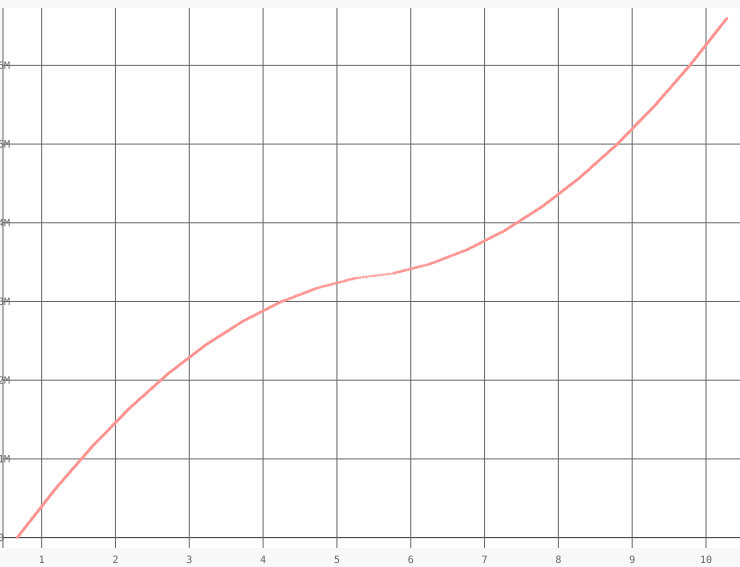
\includegraphics[angle=90]{set_a_0.5s/set_a_0_5s.png}
    \end{center}
\clearpage

\section{0.25s}
    \noindent\begin{minipage}{.45\textwidth}
    \lstinputlisting[basicstyle=\ttfamily\scriptsize,frame=none]{set_a_0.25s/tc_changes_timestamps_set_a_0.25s.out}
    \end{minipage}\hfill
    \begin{minipage}{.45\textwidth}
    \lstinputlisting[basicstyle=\ttfamily\scriptsize,frame=none]{set_a_0.25s/iperf_set_a_0.25s.out}
    \end{minipage}
    
    \begin{center}
    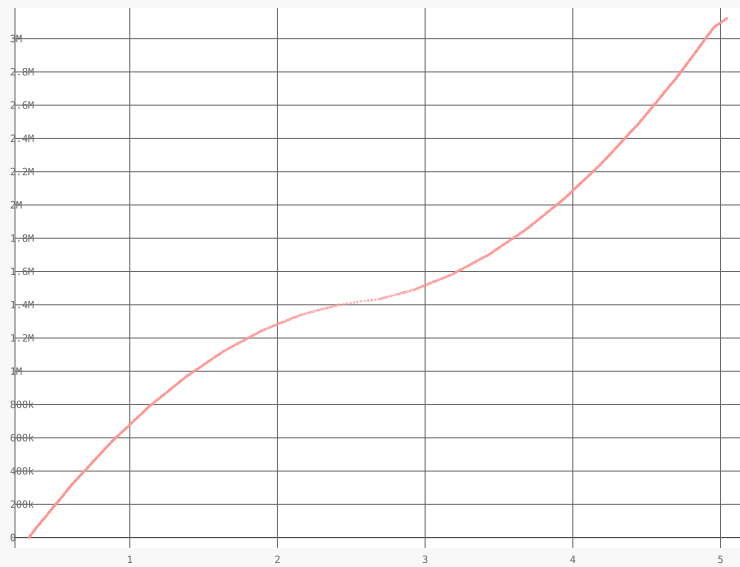
\includegraphics[angle=90]{set_a_0.25s/set_a_0_25s.png}
    \end{center}
\clearpage

\section{0.1s}
    \noindent\begin{minipage}{.45\textwidth}
    \lstinputlisting[basicstyle=\ttfamily\scriptsize,frame=none]{set_a_0.1s/tc_changes_timestamps_set_a_0.1s.out}
    \end{minipage}\hfill
    \begin{minipage}{.45\textwidth}
    \lstinputlisting[basicstyle=\ttfamily\scriptsize,frame=none]{set_a_0.1s/iperf_set_a_0.1s.out}
    \end{minipage}
    
    \begin{center}
    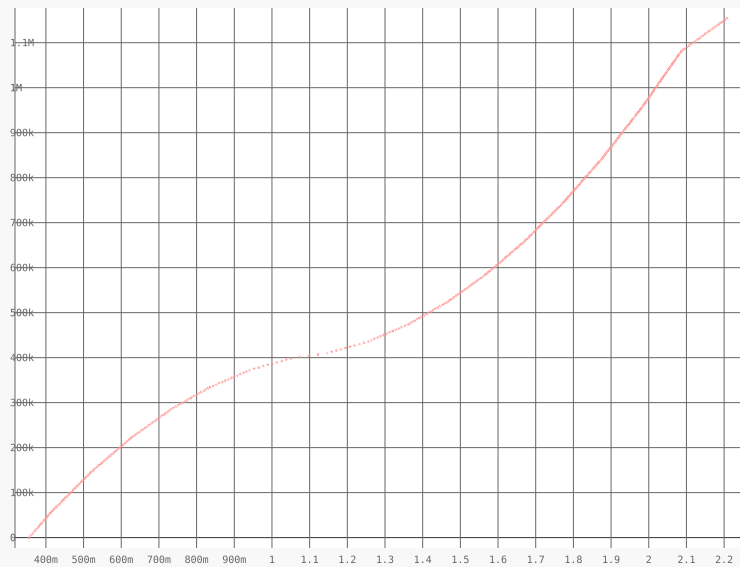
\includegraphics[angle=90]{set_a_0.1s/set_a_0_1s.png}
    \end{center}
\clearpage

\section{0.01s}
    \noindent\begin{minipage}{.45\textwidth}
    \lstinputlisting[basicstyle=\ttfamily\scriptsize,frame=none]{set_a_0.01s/tc_changes_timestamps_set_a_0.01s.out}
    \end{minipage}\hfill
    \begin{minipage}{.45\textwidth}
    \lstinputlisting[basicstyle=\ttfamily\scriptsize,frame=none]{set_a_0.01s/iperf_set_a_0.01s.out}
    \end{minipage}
    
    \begin{center}
    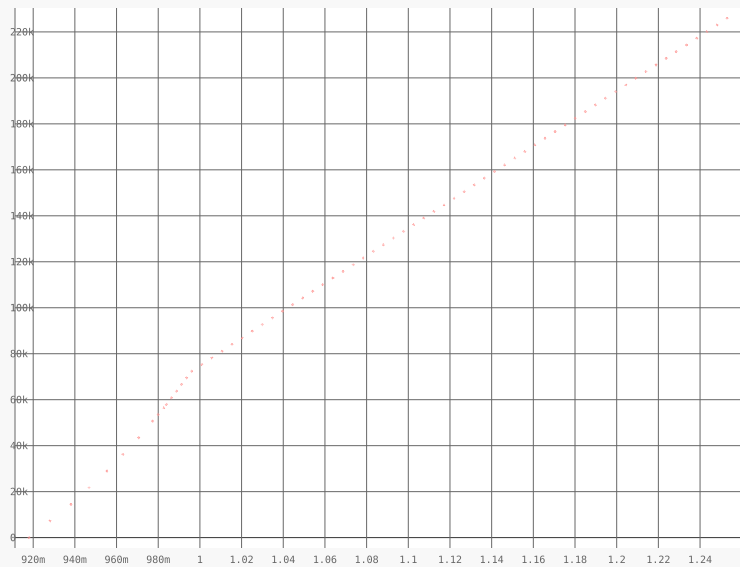
\includegraphics[angle=90]{set_a_0.01s/set_a_0_01s.png}
    \end{center}
\clearpage


%----------------------------------------------------------------------------------------

\end{document}
